\section[The Stable System]{The Stable System: Architecture of a Wrestler's World}

If sumo's mythology provided its soul and the Edo period its commercial structure, the \japterm{heya}{部屋} system—literally "room" or "fraternity house"—constitutes its skeleton. Every professional wrestler belongs to a stable, where he lives, trains, eats, and sleeps under the authority of a retired wrestler who shapes not just his technique but his entire existence. The stable is total institution and vocational school, family and factory, all compressed into a hierarchical microcosm that has remained structurally consistent for over two centuries.

Understanding the stable system is essential for any statistical analysis of sumo, because it generates many of the sport's most distinctive patterns. Wrestlers from the same stable never face each other in regular tournament bouts, creating systematic missing data. The foreign-born wrestler cap applies at the stable level, affecting recruitment strategies. Success clusters within certain stables across generations, suggesting either superior training methods or advantageous political positioning within the Japan Sumo Association. The stable is where individual athletic potential encounters institutional constraint.

\subsection{Origins: From Ronin to Heya}

The stable system emerged during the Genroku period (1688--1704) as sumo transformed from scattered rural entertainment into organized urban spectacle. Groups of wrestlers concentrated in the major cities of Edo, Osaka, and Kyoto, many of them masterless samurai—\japterm{ronin}{浪人}—who had lost their social positions and stipends with the peace established by the Tokugawa shogunate. War no longer provided employment for martial skill, but the growing merchant class in these cities had disposable income and appetite for entertainment.

These early wrestling groups self-organized under the leadership of elders who had achieved prominence in the ring. The elders welcomed wrestlers into their homes, providing lodging, meals, and training in exchange for loyalty and a share of tournament earnings. Their homes took the name \japterm{heya}{部屋} in reference to the rooms where these elders met to organize matches during tournaments. What began as pragmatic boarding arrangements gradually formalized into hereditary institutions.

The system proved profitable and was formally adopted by sumo associations in Osaka and Edo between 1757 and 1792. During the Hōreki era (1751--1764), masters began to inherit the names of their predecessors, establishing continuity across generations. A heya ceased to be merely the domain of a particular individual and became instead an institutional entity identified by an elder name—a \japterm{toshiyori kabu}{年寄株}—that could be passed down, sold, or borrowed. The stable name derives from this elder stock, creating a system where institutional identity persists even as the individuals who embody it change.

An interesting historical exception existed during the Edo period for wrestlers who benefited from the patronage of feudal lords. These \japterm{kakae-rikishi}{抱え力士}—"embraced" or "retained" wrestlers—were not formally attached to stables but instead maintained by daimyo who took the most prominent wrestlers under their wing, much as they might patronize artists or scholars. This practice faded during the Meiji period as the aristocratic class lost its wealth and influence, and by the modern era all professional wrestlers were required to belong to a stable.

\subsection{The Ichimon System: Clans Within the Association}

Stables do not exist in isolation. They organize into larger groupings called \japterm{ichimon}{一門}, typically translated as "clans" or "factions." These groups function as political alliances within the Japan Sumo Association, coordinating votes for the board of directors and organizing joint training sessions before tournaments. The ichimon system adds another layer of structure to professional sumo, creating networks of obligation and mutual support that extend beyond individual stables.

Understanding the distinction between stables and ichimon is essential: \textit{every stable must belong to one of the five ichimon}, but a stable's name does not determine which ichimon it joins. For example, Nishonoseki stable (where rising star Onosato trains) is the head stable of the Nishonoseki ichimon, which includes 16 other member stables. Meanwhile, Tatsunami stable and Kise stable (home to yokozuna Terunofuji and ozeki Kirishima respectively) are both members of the completely different Dewanoumi ichimon, despite neither having "Dewanoumi" in their stable names.

As of October 2024, there are five ichimon:

\begin{itemize}
\item \textbf{Nishonoseki ichimon} (17 stables): The largest faction, historically dominant in association politics. Led by Nishonoseki stable, members include Sadogatake, Kataonami, Hanaregoma, Hidenoyama, and others.
\item \textbf{Dewanoumi ichimon} (14 stables): Nearly equal to Nishonoseki in size and influence; together these two clans control association governance. Led by Dewanoumi stable, members include Tatsunami, Kise, Fujishima, Sakaigawa, Musashigawa, Kasugano, and others.
\item \textbf{Isegahama ichimon} (5 stables): The only clan to have never produced a chairman of the association.
\item \textbf{Tokitsukaze ichimon} (5 stables): Mid-sized faction with historical roots in Osaka sumo.
\item \textbf{Takasago ichimon} (4 stables): The smallest clan but historically prestigious, having produced numerous yokozuna.
\end{itemize}

The distribution of power is remarkably uneven. Dewanoumi and Nishonoseki each command more influence than the three smallest clans combined. This is reflected in board composition: as of 2024, the ten elected directors break down to three from Dewanoumi, three from Nishonoseki, two from Tokitsukaze, one from Takasago, and one from Isegahama. Voting for directors follows ichimon lines with striking consistency, making clan affiliation a crucial determinant of political influence.

In July 2018, the Japan Sumo Association formalized what had long been informal practice, mandating that all sumo elders must belong to one of the five ichimon. This requirement institutionalized factional politics, ensuring that stable allegiances structure not just training but governance.

The clans also organize joint training practices—\japterm{rengo-geiko}{連合稽古}—before tournaments, allowing wrestlers from affiliated stables to spar against different opponents and share techniques. These joint sessions create networks of familiarity and sometimes friendship across stable boundaries, though they also reinforce clan loyalties that can affect tournament outcomes in subtle ways.

\subsection{Stable Demographics: Growth, Peak, and Consolidation}

The number of active stables has fluctuated significantly over the modern era, shaped by regulatory changes, economic pressures, and the availability of elder stock. Table \ref{tab:stable_count} presents the historical trajectory.

\begin{table}[h]
\centering
\small
\caption{Number of Active Sumo Stables, 2006--2024}
\label{tab:stable_count}
\begin{tabular}{lcc}
\toprule
\textbf{Year} & \textbf{Stables} & \textbf{Notes} \\
\midrule
Aug 2006 & 54 & Historical peak \\
2007 & 43 & Post-regulation decline \\
2013 & 43 & Closure streak ends \\
2018 & \textasciitilde45 & Approximate \\
2024 & 46 & Current (May 2024) \\
\bottomrule
\end{tabular}
\end{table}

The peak of 54 stables in August 2006 represented the culmination of a period of expansion, driven in part by the success of foreign-born wrestlers who attracted new recruits and generated revenue. However, in September 2006—one month after the peak—the Japan Sumo Association introduced stringent new requirements for opening stables. These rules dramatically raised the qualifications needed for former wrestlers wishing to branch out and establish independent heya.

Under the new regulations, only \japterm{oyakata}{親方} (stable masters) who had spent at least 25 tournaments ranked in the titled \japterm{san'yaku}{三役} ranks (komusubi or above) or 60 tournaments in the top \japterm{makuuchi}{幕内} division could open new stables. This effectively limited stable creation to the most elite former wrestlers. Yokozuna and ozeki faced no such restrictions, but lower-ranked wrestlers suddenly found independent stable ownership nearly impossible.

In contrast, the criteria for inheriting an existing stable remained far more lenient: only 12 makuuchi or 20 juryo tournaments. This asymmetry created strong incentives for would-be stable masters to inherit or merge with existing heya rather than strike out independently.

The consequences were immediate. Over the next six years, no new stables opened while eleven folded, bringing the total down to 43 by 2013. The closure streak finally ended in April 2013 when former yokozuna Musashimaru—easily meeting the new requirements—opened Musashigawa stable. Since then the number has stabilized around 45--46, suggesting the current regulatory regime has established an equilibrium.

This consolidation has implications for the sport's competitive structure. Fewer stables means larger rosters per stable, concentrating training resources but also potentially reducing the diversity of coaching styles and strategic approaches available to young wrestlers. It also makes elder stock more valuable, as the pathways to stable ownership have narrowed considerably.

\subsection{The Toshiyori Kabu: Elder Stock as Scarce Resource}

To understand who can own a stable, one must first understand the \japterm{toshiyori kabu}{年寄株} system. These "elder stocks" are shares in the Japan Sumo Association, limited to exactly 105 since 1927. A retired wrestler cannot become an elder—and therefore cannot coach or own a stable—without acquiring one of these shares.

The requirements for kabu acquisition are stringent:

\begin{itemize}
\item \textbf{Japanese citizenship}: Since 1976, foreign-born wrestlers must renounce their original nationality and naturalize as Japanese citizens to acquire elder stock. This requirement has profound implications for Mongolian, European, and other foreign-born wrestlers who might otherwise transition into coaching.
\item \textbf{Rank achievement}: Wrestlers must have either competed in at least one tournament at san'yaku rank (komusubi or above), or 20 tournaments in the top makuuchi division, or 30 tournaments as a \japterm{sekitori}{関取} (salaried wrestler in the top two divisions). In November 2013, rules were modified to allow membership after 28 sekitori tournaments in certain circumstances.
\item \textbf{Clean disciplinary record}: Wrestlers with serious infractions are typically barred from elder stock acquisition.
\end{itemize}

The value of these shares is extraordinarily high, though official prices are not publicly disclosed. Anecdotal reports suggest figures in the hundreds of millions of yen (several million US dollars). The scarcity is by design: limiting elder stock to 105 ensures that only the most successful wrestlers transition into the association's governance and coaching ranks.

Kabu can be owned, borrowed, or inherited. Ownership conveys full rights and status; borrowers occupy the lowest tier of the elder hierarchy, cannot advance in the association's administrative structure, and crucially, \textit{cannot own a stable}. This creates a two-tier system among elders, with stable ownership reserved for those wealthy or successful enough to acquire their own shares.

When a stable master retires at the mandatory age of 65, he must transfer his kabu and stable to a successor. This transition often follows familial lines—sons-in-law are common successors—but can also go to prominent wrestlers from within the stable or be sold to outsiders. The mechanics of these transfers structure much of sumo's behind-the-scenes politics, as ambitious wrestlers maneuver for positions that will allow them to inherit or purchase valuable elder names.

\subsection{Opening a Stable: Branching and Succession}

There are two pathways to stable ownership: \textit{branching out} (\japterm{shinhatsubai}{新発売}) to create a new independent stable, or \textit{inheriting} an existing one. As described above, the September 2006 regulatory changes made branching extraordinarily difficult, requiring 25 san'yaku tournaments or 60 makuuchi tournaments for anyone below the rank of ozeki. Inheritance requires only 12 makuuchi or 20 juryo tournaments, creating a powerful incentive toward succession rather than independence.

The practical requirements extend beyond rank achievement:

\begin{itemize}
\item \textbf{Marriage}: A stable master must be married. The reasoning is institutional: a stable cannot be run by an \japterm{oyakata}{親方} alone. The stable master's wife—the \japterm{okamisan}{女将さん}—functions as the stable's primary administrator, managing finances, organizing supporter functions, overseeing daily operations, and often handling all money flowing through the stable. Tradition dictates that the oyakata acts as "father" to the wrestlers while the okamisan serves as "mother," creating a familial structure essential to the total institution model.
\item \textbf{Financial resources}: Opening or maintaining a stable requires substantial capital. The oyakata must secure a physical location with training facilities (\japterm{keikoba}{稽古場}), living quarters for wrestlers, and family residence. He must also fund daily operations: food, utilities, equipment, medical care, and salaries for any staff. While higher-ranked wrestlers within the stable (sekitori) receive salaries from the association, lower-ranked wrestlers receive only small stipends, and their living expenses fall on the stable.
\item \textbf{Elder stock ownership}: As noted, only those who own (rather than borrow) their toshiyori kabu can establish or inherit stables.
\item \textbf{Clan affiliation}: Since 2018, all elders must belong to one of the five ichimon, effectively requiring stable masters to align with a political faction and participate in its governance structures.
\end{itemize}

A stable is always named after the toshiyori kabu owned by its head coach, not after the individual himself. When Hakuho, the 69th yokozuna, acquired the Miyagino elder stock and inherited Miyagino stable in 2021, the stable retained its name even though Hakuho was its new master. This system ensures institutional continuity across generations of leadership.

\subsection{Recruitment: The Search for New Talent}

A stable's survival depends on continuously recruiting young wrestlers. Stable masters maintain informal networks throughout Japan, attending local tournaments and cultivating relationships with coaches who can identify promising talent. Scouts look for specific physical attributes—historically at least 173 cm tall and 75 kg, though requirements loosened in 2023—and more importantly, frame size suggesting potential for growth. The ideal recruit is a teenager with a large skeletal structure who can develop under the stable's intensive training and feeding regimen.

Reputation matters enormously. Stables that recently produced yokozuna or ozeki attract ambitious recruits whose families believe that lineage indicates superior training. Stables in decline face recruitment crises, creating vicious cycles where lack of talent prevents success, which deters future recruits.

Foreign recruitment transformed the landscape beginning in 1992 when Oshima Oyakata traveled to Mongolia and recruited six wrestlers trained in \textit{bökh}, Mongolian traditional wrestling.\cite{diplomat2020mongolia} This proved consequential: Mongolian wrestlers subsequently dominated professional sumo, with Asashoryu and Hakuho becoming yokozuna and winning nearly every tournament between 2006 and 2016. The one-foreign-wrestler-per-stable cap (implemented 2002) made each foreign recruitment decision high-stakes—a single successful Mongolian could transform a stable's prospects for a decade.

Parallel to scouting raw talent, stables recruit accomplished amateur champions through the \textit{makushita tsukedashi} system (established 1972). Originally, amateur title winners could start at makushita 15 or even makushita 10, a substantial advantage. Only three wrestlers ever qualified for makushita 10: Endo, Mitakeumi, and Onosato.\cite{jasumo2024tsukedashi} In 2023, the association reformed this system, lowering the starting rank to makushita 60 but expanding eligibility.\cite{tachiai2023reforms} Eleven wrestlers debuted via this pathway in 2024—more than double the historical pace—shifting recruitment strategy toward accomplished university wrestlers rather than raw teenage prospects.

Despite sumo's current popularity, recruitment has collapsed. Spring 2024 saw only 27 new recruits, the lowest since 1973, compared to 160 in 1992.\cite{japantimes2024recruitment} Japan's demographic decline, competing career opportunities, economic precarity (only juryo wrestlers receive salaries), injury risk, and periodic scandals all deter modern teenagers from choosing sumo. The recruitment crisis affects stables unequally: elite stables with championship pedigrees and university connections continue attracting talent, while smaller stables face existential threats, creating widening inequality in the stable system.

\subsection{Stable Closures and Mergers}

While much attention focuses on stable openings, closures are equally important to understanding system dynamics. Stables close for several reasons: the oyakata's mandatory retirement at 65 without a suitable successor; financial insolvency; scandal or disciplinary action; or voluntary merger with another heya.

Recent high-profile closures illustrate the range of causes:

\begin{itemize}
\item \textbf{Takanohana stable} (October 2018): Closed following a power struggle between former yokozuna Takanohana and the association's leadership. All wrestlers transferred to Chiganoura stable. This closure was fundamentally political, ending one of the most successful and visible stables of the modern era.
\item \textbf{Izutsu stable} (September 2019): Closed when the oyakata reached retirement age without a successor willing to inherit. Wrestlers moved to Michinoku stable. This represents the demographic challenge facing smaller stables: without a pipeline of successful wrestlers capable of acquiring elder stock, the stable dies with its master.
\item \textbf{Nakagawa stable} (July 2020): Closed due to the oyakata's health issues. Wrestlers were distributed among multiple stables rather than transferred en masse, suggesting either the lack of a suitable inheritor or strategic decisions by the association about wrestler placement.
\item \textbf{Miyagino stable} (March 2024): Forcibly closed by the Japan Sumo Association following a scandal involving physical abuse by wrestler Hokuseihō and subsequent punishment of stable master Hakuhō. This was particularly dramatic given Hakuhō's status as arguably the greatest wrestler in sumo history, demonstrating that even the most prestigious stables are not immune to closure for disciplinary reasons.
\end{itemize}

These closures reflect the precariousness of institutional survival in professional sumo. A stable requires not just financial resources and successful wrestlers, but also political capital, clean governance, and a viable succession plan. The 2006 regulations made this even more challenging by restricting who could branch out independently, concentrating stable ownership among an elite tier of former champions.

Some stables have extraordinary longevity. Tatsunami stable, founded in 1876 (current incarnation from 1915), has operated for over a century and produced multiple yokozuna, including the legendary Futabayama and Haguroyama in the 1930s. Its persistence demonstrates that institutional quality can compound across generations, as successful training produces champions who become oyakata who train the next generation of champions.

\subsection{Daily Life: Hierarchy, Training, and Total Institution}

The stable is not merely a training facility; it is a total institution that structures every aspect of a wrestler's existence. Wrestlers live communally under a rigid hierarchical system that determines where they sleep, what they eat, when they train, and whom they serve.

\begin{figure}[h]
\centering
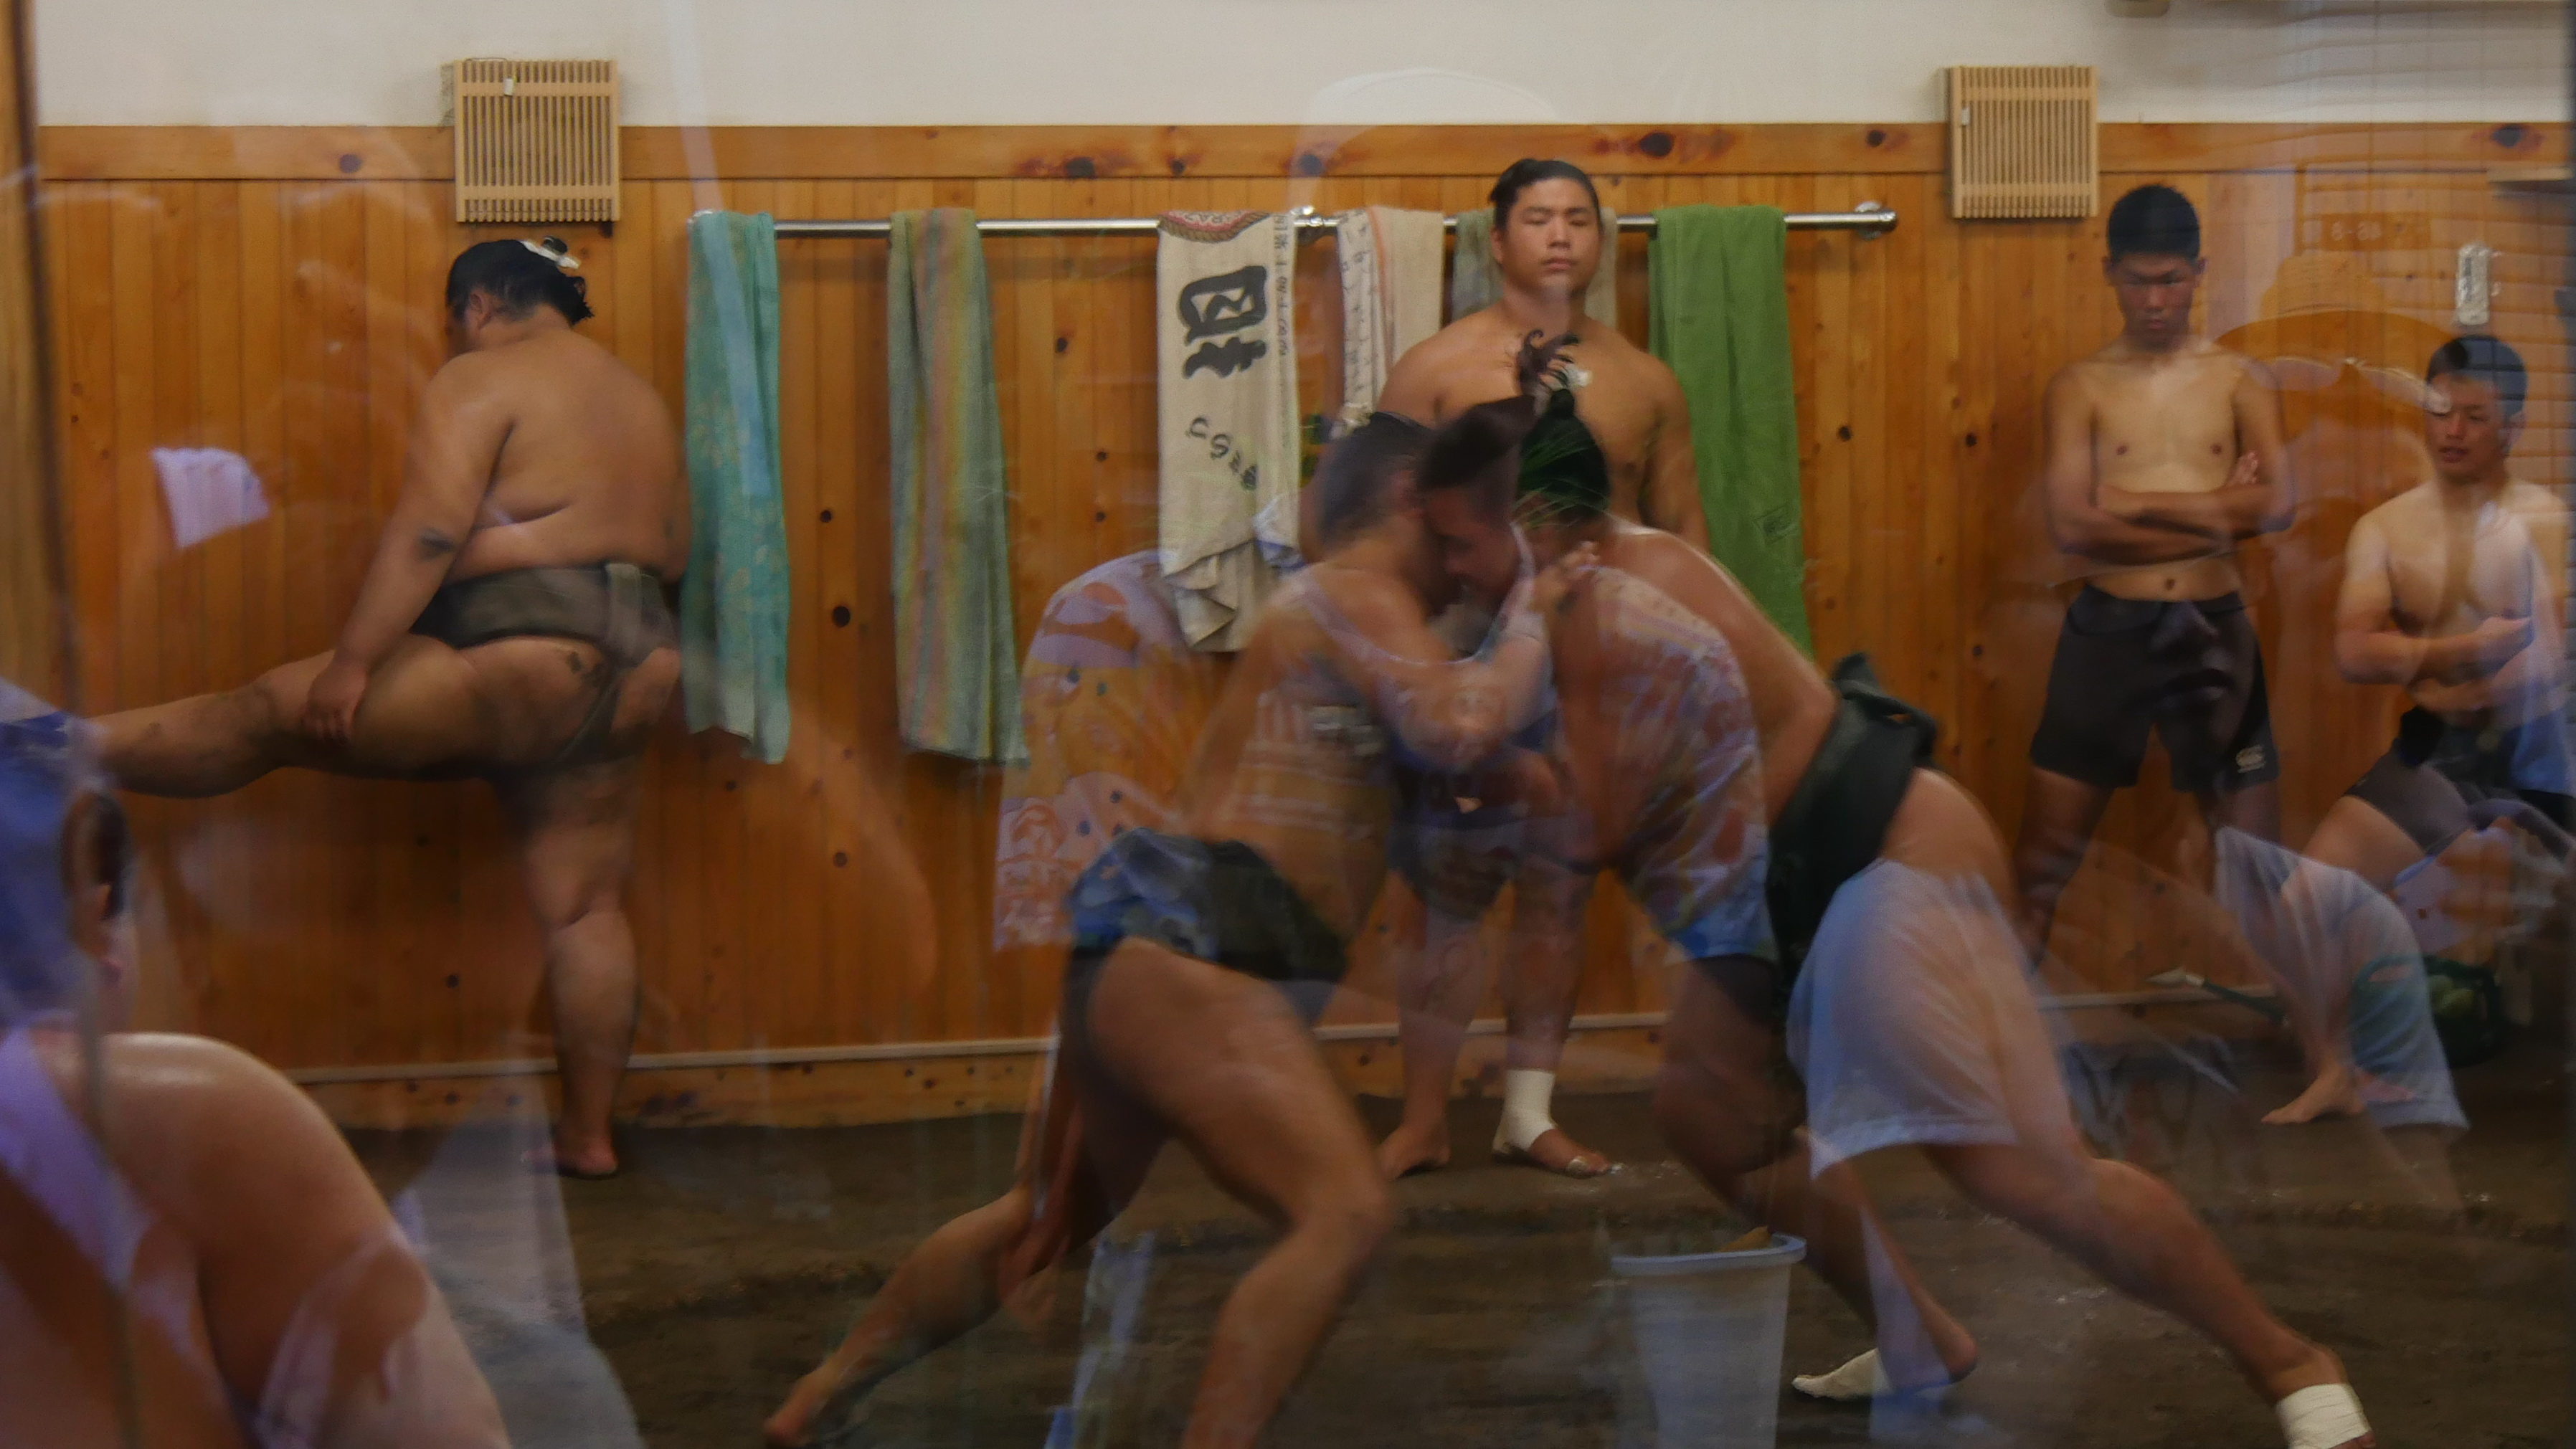
\includegraphics[width=0.9\textwidth]{images/ch01_history/sumo_training.jpg}
\caption{Morning training session at a Tokyo sumo stable, 2014. Junior wrestlers practice under the oyakata's supervision in the keikoba (training ring). Photo: Public domain via Wikimedia Commons.}
\label{fig:sumo_training}
\end{figure}

\subsubsection{The Hierarchy: Sekitori and Wakaisho}

Wrestlers divide into two castes with radically different lived experiences:

\begin{itemize}
\item \textbf{Sekitori} (\japterm{sekitori}{関取}): Wrestlers in the top two divisions (makuuchi and juryo). These are salaried employees of the Japan Sumo Association, earning substantial monthly stipends that increase with rank. Sekitori enjoy private rooms, personal attendants drawn from lower-ranked wrestlers, freedom to marry, the right to wear silk mawashi and elaborate kesho-mawashi during ring-entering ceremonies, and relative autonomy in daily life.
\item \textbf{Wakaisho} (\japterm{wakaisho}{若い衆}): All other wrestlers, comprising the vast majority of stable residents. These men are unsalaried, receiving only small monthly stipends (often around 100,000 yen or roughly \$700 USD). They share cramped sleeping quarters, often sleeping in groups on the floor of common rooms. They perform all stable chores: cooking, cleaning, laundry, and serving as personal attendants to sekitori. They cannot marry without permission, which is rarely granted to anyone below juryo rank.
\end{itemize}

This division is absolute. A wrestler promoted from makushita (the highest unsalaried division) to juryo undergoes an instant transformation in status, moving from shared quarters to a private room, from servant to master. Conversely, demotion from juryo to makushita means loss of salary, privacy, and autonomy—a fall that often precipitates retirement.

\subsubsection{The Daily Schedule}

A typical day at a sumo stable follows an unvarying pattern designed to maximize training intensity while building group cohesion:

\begin{enumerate}
\item \textbf{5:00--6:00 AM}: Wrestlers rise before dawn. Junior wrestlers wake earlier to prepare the training area and begin chores.
\item \textbf{6:00--11:00 AM}: Morning practice (\japterm{keiko}{稽古}) begins. Training occurs on an empty stomach, a practice believed to increase intensity and mental toughness. Sessions last 3--5 hours without breaks, consisting of repetitive drills, practice bouts (\japterm{butsukari-geiko}{ぶつかり稽古}), and full-intensity matches between wrestlers. The oyakata observes, offering corrections and occasionally demonstrating techniques. Higher-ranked wrestlers train first while lower-ranked wrestlers wait their turn, reinforcing hierarchy through every aspect of practice.
\item \textbf{11:00 AM--12:00 PM}: While sekitori bathe and relax, junior wrestlers prepare the first meal of the day.
\item \textbf{12:00--2:00 PM}: The communal meal, centered on \japterm{chanko-nabe}{ちゃんこ鍋}, a protein-rich stew designed to help wrestlers gain weight. Chanko is not a single recipe but a category of hearty stews, often including chicken, fish, tofu, vegetables, and broth, accompanied by rice and side dishes. Junior wrestlers serve sekitori first, eating only after their seniors are satisfied. This meal is enormous, often constituting 3,000--5,000 calories.
\item \textbf{2:00--5:00 PM}: Mandatory nap time. Sleeping after the massive midday meal promotes weight gain and recovery. Sekitori sleep in private rooms while junior wrestlers share common spaces.
\item \textbf{5:00--8:00 PM}: Free time for sekitori; junior wrestlers continue chores, prepare the evening meal, and handle stable maintenance.
\item \textbf{8:00--9:00 PM}: Evening meal, again communal and hierarchical. The meal is substantial but less overwhelming than lunch.
\item \textbf{9:00--10:00 PM}: Wrestlers retire, with junior wrestlers ensuring the stable is clean and secure before sleeping.
\end{enumerate}

This schedule repeats with almost no variation, six days per week, throughout the year except during tournament periods when training gives way to competition. The monotony is intentional, creating a structured environment that minimizes external distractions and focuses attention entirely on sumo.

\subsubsection{The Role of the Okamisan}

The stable master's wife occupies a position of extraordinary authority and responsibility. She manages finances, often controlling all money flowing through the stable including wrestlers' savings. She organizes supporter club functions, dinners with patrons and sponsors, and recruitment efforts. She oversees the kitchen and teaches junior wrestlers basic life skills. In some cases, when an oyakata is in poor health, the okamisan even supervises training.

Her role extends to counseling young wrestlers through personal crises, mediating disputes, and maintaining stable morale. Without an effective okamisan, many stables would struggle to function. This is why marriage is mandatory for stable masters: the institution requires both father and mother figures to operate.

The okamisan's power is informal but pervasive. She cannot hold official rank in the association, but her influence within the stable often rivals or exceeds that of assistant coaches. Former wrestlers' wives bring their own networks and expertise, creating dynasties where sumo knowledge passes through both male and female lines.

\subsection{Economics and Sustainability}

Running a stable is expensive. The oyakata must secure and maintain a physical facility, often in expensive urban areas like Tokyo where land values are exorbitant. He must feed dozens of young men who consume enormous quantities of food. He must pay for medical care, equipment, utilities, transportation to tournaments, and salaries for any staff beyond the wrestlers themselves.

Revenue comes from several sources:

\begin{itemize}
\item \textbf{Association stipends}: The JSA provides financial support to stables, though the amounts are modest relative to operating costs.
\item \textbf{Sekitori salaries shared with the stable}: While sekitori receive salaries directly, they traditionally contribute a portion back to the stable that trained them, particularly for major expenses.
\item \textbf{Tournament bonuses}: When a stable's wrestler wins or performs exceptionally, the stable receives prize money.
\item \textbf{Supporter associations} (\japterm{koen-kai}{後援会}): These are groups of fans and patrons who provide financial support to stables in exchange for access to wrestlers, special events, and social prestige. Wealthy supporters can contribute millions of yen annually, making the cultivation of these relationships essential to stable survival.
\item \textbf{Corporate sponsorships}: Some stables secure sponsorships from businesses seeking association with sumo's traditional prestige.
\item \textbf{Personal wealth}: Many oyakata subsidize their stables from personal funds, particularly in the early years before a stable's wrestlers reach salaried ranks.
\end{itemize}

The economic model is precarious. A stable with no sekitori operates at a loss, dependent entirely on supporter generosity and the oyakata's resources. A stable with multiple high-ranking sekitori can be profitable, but success in the ring is unpredictable. This creates strong incentives to recruit promising young talent and intense pressure to develop them quickly.

The foreign-born wrestler restriction—one per stable—affects economics significantly. Foreign wrestlers, particularly Mongolians, have dominated the top ranks in recent decades. A stable fortunate enough to recruit a successful foreign wrestler gains enormous financial advantage, but the one-per-stable cap prevents any heya from monopolizing foreign talent. This rule, implemented in February 2002, replaced an earlier system allowing two foreigners per stable, reflecting association concerns about foreign dominance.

\subsection{Training Philosophy and Stable Culture}

Not all stables train identically. While the basic structure remains consistent—morning practice, communal meals, hierarchical living arrangements—stable masters develop distinct philosophies that shape their wrestlers' styles and career trajectories.

Some stables emphasize technical precision, drilling specific techniques until they become reflexive. Others prioritize raw physicality, focusing on strength conditioning and aggressive practice bouts. Some oyakata are hands-on, participating actively in daily training; others observe and correct from a distance. These differences create identifiable stable styles: Miyagino stable under Hakuhō was known for technical sophistication and strategic patience; Takasago stable has historically produced powerful, aggressive wrestlers.

The psychological environment varies as well. Some stables cultivate intense competition among wrestlers, encouraging rivalry and aggressive internal hierarchy. Others emphasize cooperation and mutual development. Some oyakata rule through fear and physical punishment; others lead through mentorship and positive reinforcement. These cultural differences affect not just wrestler development but also retention—stables with particularly harsh cultures see higher dropout rates among young recruits, though those who survive may be more resilient.

\subsection{Famous Stables and Their Legacies}

Certain stables have shaped sumo history through sustained excellence or cultural impact:

\begin{itemize}
\item \textbf{Tatsunami stable}: One of the oldest continuous stables, founded 1876. Produced yokozuna Futabayama (1930s), who achieved an unprecedented 69-bout winning streak that stood for decades as sumo's most legendary record, and Haguroyama, who ended Dewanoumi stable's long dominance. Tatsunami remains active and aligned with Dewanoumi ichimon.
\item \textbf{Takasago stable}: Historically prestigious, produced seven yokozuna including Asashōryū and Asahifuji. Also produced Konishiki, the first non-Japanese ozeki (Hawaiian). In September 2025, Takasago saw three sekitori promotions in a single tournament, the first time this had occurred for any stable since Sadogatake in September 1979, demonstrating its continued competitiveness.
\item \textbf{Miyagino stable}: Home to Hakuhō, arguably the greatest wrestler in sumo history with 45 tournament championships. Hakuhō became stable master in 2021 after acquiring Miyagino elder stock, but the stable was forcibly closed in March 2024 following the Hokuseihō abuse scandal. Its closure exemplifies how quickly institutional prestige can collapse under disciplinary pressure.
\item \textbf{Dewanoumi stable}: Historically dominant in the early 20th century, the stable name became synonymous with sumo excellence and its descendants form the second-largest ichimon. Though the original Dewanoumi stable closed, its lineage persists through affiliated stables.
\item \textbf{Azumazeki stable}: Founded by Takamiyama (the first foreign makuuchi wrestler), became famous for Hawaiian recruitment pipeline that produced yokozuna Akebono and Musashimaru. Demonstrates how a single successful foreign wrestler could transform a stable's trajectory by leveraging ethnic and geographic networks.
\end{itemize}

These stables illustrate how institutional success compounds across generations. A stable that produces a yokozuna gains prestige that attracts recruits, some of whom become champions who eventually return as coaches, perpetuating excellence. Conversely, stables without recent success struggle to break into the elite tier, lacking the reputation needed to recruit top talent.

Table \ref{tab:stable_success} presents success metrics for selected prominent stables, measured by total yokozuna produced (all-time) and current sekitori count (as of 2024).

\begin{table}[h]
\centering
\small
\caption{Success Metrics for Selected Sumo Stables}
\label{tab:stable_success}
\begin{tabular}{lccc}
\toprule
\textbf{Stable} & \textbf{Yokozuna} & \textbf{Status} & \textbf{Ichimon} \\
\midrule
Takasago & 7 & Active & Takasago \\
Tatsunami & 2+ & Active & Dewanoumi \\
Miyagino & 1 (Hakuhō) & Closed 2024 & -- \\
Kokonoe & 3 & Active & Takasago \\
Isegahama & 4 & Active & Isegahama \\
\bottomrule
\end{tabular}
\end{table}

\subsection{The Stable as Data-Generating Institution}

For researchers, the stable system creates both opportunities and complications. On one hand, it provides natural clustering for hierarchical models: wrestlers within a stable share training methods, coaching, dietary practices, and competitive strategies, making stable affiliation a crucial random effect in any outcome model. Stable-level analysis can reveal which training philosophies produce superior results and whether success concentrates due to coaching quality or simply talent recruitment.

On the other hand, the same-stable non-competition rule creates systematic missing data. When estimating wrestler strength using rating systems like Elo or Glicko, we never observe within-stable matchups, which can bias estimates if stable membership correlates with wrestler quality. The missing data is not random: strong stables accumulate strong wrestlers, but those wrestlers never face each other in regulation bouts (except rare playoff scenarios), meaning our most informative potential comparisons remain unobserved.

The foreign wrestler cap also complicates analysis. If Mongolian wrestlers are systematically stronger (as recent tournament results suggest), then stables lucky enough to recruit successful Mongolians enjoy enormous competitive advantages, but each stable can have only one. This creates winner-take-all dynamics at the recruitment stage, where a single high-value foreign recruit can determine a stable's trajectory for a decade.

Finally, the ichimon system introduces political economy considerations. Wrestlers from aligned stables might—consciously or unconsciously—adjust effort when facing opponents from allied clans, particularly in tournaments where outcomes affect promotion decisions. While match-fixing scandals have erupted periodically, the more subtle question is whether factional loyalty creates detectable patterns in bout outcomes even absent overt collusion. These are empirical questions that later chapters will address.

\subsection{Modern Challenges and Evolution}

The stable system faces pressures that would have been unimaginable a century ago. Declining birth rates in Japan mean fewer potential recruits. The sport's grueling demands and hierarchical culture deter many young men who have less brutal career options available. Scandals involving hazing, physical abuse, and financial impropriety have damaged sumo's public image, making parental consent for teenage recruitment harder to obtain.

The 2006 regulatory tightening, while intended to preserve quality by restricting stable ownership to elite former wrestlers, has also created succession crises. Smaller stables without a pipeline of champions struggle to find qualified inheritors, leading to closures and consolidation. The current equilibrium of around 46 stables may represent a new normal, with total stable count unlikely to return to historical peaks absent regulatory reform.

Technological change also affects traditional stable life. Wrestlers now use smartphones, access social media, and maintain public profiles in ways that would have been impossible in earlier eras. This connectivity undermines the total institution model, introducing external influences and comparisons that can destabilize stable hierarchy. Some oyakata have banned phones during training periods; others embrace technology as recruitment and fan engagement tools.

The foreign wrestler debate continues to evolve. Mongolian dominance has prompted periodic calls for tighter restrictions, met by counterarguments that foreign wrestlers have revitalized interest in the sport and that nationalist restrictions betray sumo's claim to be "Japan's national sport" open to all. The citizenship requirement for elder stock means successful foreign wrestlers face a profound choice: remain citizens of their birth countries and retire completely from sumo after their wrestling careers end, or naturalize as Japanese and potentially become stable masters themselves. Hakuhō chose the latter path, renouncing Mongolian citizenship to acquire Miyagino elder stock, though his stable's subsequent closure demonstrates that even full assimilation provides no guarantee of institutional survival.

The stable system has persisted for over two centuries because it solves fundamental problems: how to train athletes in an specialized combat sport, how to organize tournaments among wrestlers of radically different skill levels, how to preserve institutional knowledge across generations, and how to maintain cultural continuity in a society that has otherwise modernized beyond recognition. Whether it will persist another two centuries depends on its ability to adapt to demographic decline, technological disruption, and changing cultural expectations about hierarchy and authority. For now, it remains the indispensable core of professional sumo, shaping every aspect of the sport that any statistical model must account for.
